\section{Aide à la Décision Multi-Critère}
\label{sec:ADMC}
Nous ne pourrons dans cette section que traiter partiellement du domaine de la décision multi-critère.
Nous ne traiterons donc pas de toutes les propriétés que nous avons pu listé en littérature\footnote{Notamment grâce à l'ouvrage de \citeauthor{bouyssou_evaluation_2006}~\cite{bouyssou_evaluation_2006}}
(Anonymat,
Indifférence,
Incomparabilité,
Intransitivité,
Asymétrie,
Exhaustivité,
Neutralité,
Réactivité positive,
Indépendance des alternatives insignifiantes).
%Anonymity,
%Indifference,
%Incomparability,
%Intransitivity,
%Asymmetry,
%Completeness,
%Neutrality,
%Positive Responsiveness,
%Independence of Irrelevant Alternatives
De même les interactions des divers champs théoriques sont nombreuses (théorie de la mesure conjointe,
théorie de la décision,
théorie du choix social,
théorie de l'utilité,
la théorie des jeux,
théorie de la «rationalité limitée»,
théorie de la significativité,
théorie des probabilités,
%théorie de la Valeur Multi-Attribut,
la théorie des graphes).
%conjoint measurement theory,
%decision theory,
%Social Choice Theory,
%utility theory,
%game theory,
%"bounded rationality" theory,
%meaningfulness theory,
%probability theory,
%Multi-Attribute Value Theory,
%graph theory
Sans pouvoir être exhaustif, nous tenterons d'apporter un éclairage suffisamment large et important pour l'articulation logique de notre travail et le développement méthodologique de l'\gls{ACV}.
%??????????
%
%Incomparabilité
%
%reprendre l'ensemble des propriétés
%
%Anonymity,
%Indifference,
%Incomparability,
%Intransitivity,
%Asymmetry,
%Completeness,
%Neutrality,
%Positive Responsiveness,
%Independence of Irrelevant Alternatives
%
%xxxxxxxxxxxxxxxxxx
%
%interaction de champ théoriques
%
%conjoint measurement theory
%decision theory
%Social Choice Theory
%utility theory
%game theory
%"bounded rationality" theory
%meaningfulness theory
%probability theory
%Multi-Attribute Value Theory
%graph theory
%
%??????
%
%Ça va faire trop gros
\subsection{Multi-dimensionnalité et assistance}

%à mettre ailleurs
%La décision revêt toutefois une dimension subjective inaliénable aux activités humaines.
La prise en compte de grandeurs différentes par leurs natures et les objets qu'elles qualifient implique des précautions nécessaires pour leurs déterminations et leurs exploitations.

Les limites cognitives de l'homme ne doivent pas être ignorées.
Elles font partie des bornes de notre rationalité sans assistance.
S'il s'agit de croiser un grand nombre d'informations sur une même analyse, des grandeurs différentes par nature, hétérogènes en unité, l'assistance de techniques numériques est requise.
Ceux sont les \glspl{ADMC}, les outils d'\acrlong{ADMC}.
En effet prendre en compte plus d'une dizaine de \emph{pièces d'information nouvelles} ne nous est pas possible.
L'ordre de grandeur de la capacité de charge de la mémoire de travail est de 4 voir 3 éléments seulement, d'après \citeauthor{farrington_seven_2011}~\cite{farrington_seven_2011}.
Il n'est donc pas surprenant de voir cette problématique de la décision multi-critère émerger en psychologie\footnote{CF. l'introduction de \citeauthor{ishizaka_review_2011} dans le cadre de sa revue sur l'AHP et la mention des psychologistes "Thurstone, 1927; Yokoyama, 1921 ; Fechner, 1860 ; Stevens, 1957"~\cite{ishizaka_review_2011}}.

Il n'est pas étonnant non plus au regard de la complexité des situations de prise de décision de voir croître le nombre de publications, dans la littérature environnementale, sur les Méthodes d'Aide (ou d'Analyse) à la (de) Décision Multi-Critère (ADMC ou MCDA en littérature anglophone), tel que le présentent \citeauthor{huang_multi-criteria_2011}~\cite{huang_multi-criteria_2011}.
La valeur totale, une part d'environ \textbf{2~\%}), elle, pourra toutefois choquer pour le lecteur ayant une connaissance globale du premier chapitre de cette thèse.
% [htbp] ici si possible, haut ou bas de page sinon, et si c'est trop grand créer une page. S'il n'y a pas ``p'' ça fonce vers la fin de la section ou du chapitre

%\colorbox{red}{à confirmer suivant juriste, mais l'utilisation du graphe m'est interdit je pense.}

%\begin{figure}[htbp]
%\begin{center}
%%\begin{figure}[r]
%\includegraphics[width=12cm]{/home/rudy/Documents/rudy/01_These/11_production/01_COMMUNICATION/figures_extraites/HUANG2011_croissance_MCDA_environnement.pdf}
%\caption{Ratio des publications environnementales traitant de l'\gls{ADMC}. Figure extraite de \cite{huang_multi-criteria_2011}.}
%%\end{figure}
%\label{fig:Croissance_ADMC-Environnement}
%\end{center}
%\end{figure}
Les dimensions sociales économiques et culturelles adjointes à la dimension environnementale en complément de l'\gls{ACV}, doivent toutes recevoir un traitement particulier.
Pour intégrer la subjectivité intrinsèque d'une étude mêlant ces attributs hétérogènes, il faut à minima que le traitement soit transparent.
La complexité sur ce plan peut être combattue.
L'adoption de lignes directrices claires quant à la sélection, la hiérarchie, aux poids des indicateurs suivis (chartes, normes, programme de règles communes~\ldots) et au traitement que subiront ceux-ci, y contribuerait.
Cela ne serait cependant efficace que \emph{dans la mesure que tous cela soit librement accessible et aisément 
%à des sélections, hiérarchies, pondérations ou règles définies
employable et modifiable par un utilisateur quelconque pour ne pas dépendre de ces lignes directrices}.

Par ailleurs, la consultation des parties-prenantes est capitale pour la mise en place de ces lignes directrices.
Si le traitement ne correspond pas à leurs attentes, l'analyse ne sera pas considérée.

De plus, le jugement opéré sur les informations présentées doit être décrit \emph{exhaustivement} afin de garantir la reproductibilité de la décision.
La description du processus peut également servir de justification en cas de contestation, critique et autres attaques.

La prise de décision multi-critère dans le cadre de l'\gls{ACV} %par outils numériques
est décrite par les travaux de \citeauthor{rowley_aggregating_2012}~\cite{rowley_aggregating_2012}.
Ceux-ci visent à éclairer la sélection des méthodes d'\gls{ADMC} suivant le problème traité et son contexte. %~\cite{rowley_aggregating_2012}.
Les classifications des méthodes d'analyse multi-critère sont variées, tel que le montrent \citeauthor{guitouni_tentative_1998} ainsi que la revue de \citeauthor{herva_review_2013}~\cite{herva_review_2013,guitouni_tentative_1998}.

Après une présentation des catégories, nous observerons les caractéristiques mathématiques centrales de ces outils. Nous présenterons ensuite succinctement certaines méthodes employées en nous attardant sur la question de la consistance.
\subsection{Méthodes d'ADMC}
% xxxxxxxxxxxxxxxxxxxxxxxxxxxxxxxxxxxxxxxxxxxxxxxxx
% %   ziout_holistic_2014
% 
%EXEMPLE APPLICATION DÉTERMINATION DE L'IMPORTANCE (HORS \gls{ACV})
%%  vaidya_analytic_2006,
%	Analytic hierarchy process: An overview of applications
%% saaty_fundamentals_2004,
%	Fundamentals of the analytic network process?Dependence and feedback in decision-making with a single network
%% saaty_making_2005,
%	Making and validating complex decisions with the {AHP}/{ANP}
%	
%	As the goal is to determine \emph{one} indicator (the relative weight of the attribute), we selected a type 1 method.
%	Furthermore, the extension to LGDM (large group decision making) has been studied with the use of AHP~\cite{liu_method_2016}.
%	This in the perspective of integrating more widely stakeholders values and preferences was important.
% xxxxxxxxxxxxxxxxxxxxxxxxxxxxxxxxxxxxxxxxxxxxxxxxx

Suivant la classification adoptée par \citeauthor{rowley_aggregating_2012} il existe trois approches d'ADMC~\cite{rowley_aggregating_2012}~:
\begin{itemize}
\item Élémentaires (seuil veto, hiérarchie, somme pondérée)
\item Interactives (interaction répétée des parties-prenantes)
\item Qui utilisent une \gls{PAMC}\footnote{Nous considérons que la somme pondérée est une agrégation de type 1.}
\end{itemize}
Les deux familles principales de procédures d'agrégation sont dites~:
\begin{itemize}
\item de Type 1, ou encore appelé opérationnelle de type 1, signifiant une agrégation complète : \emph{celles basées sur un critère de synthèse}
\item de Type 2, ou encore appelé opérationnelle de type 2, signifiant une agrégation partielle : \emph{celles basées sur la synthèse d'un système relationnel de préférence (sur-classement)}
\end{itemize}

%? développer type 1 ?
%lister autres travaux ayant sélectionné ce type méthodes

L'incertitude caractéristique de l'exercice de l'\gls{ACV} conduit à sélectionner soit un outil avec indifférence ou avec préférence faible.
La prise en compte de l'incertitude donne potentiellement lieu à des comparaisons non-strictes.
Là où les préférences strictes sont obtenues par l'emploi de \textit{critères vrais}, une plage d'indifférence et la préférence floue sont obtenues respectivement par \textit{quasi-critère} ou \textit{pseudo-critère}.
Mais introduisons quelques peu ces notions théoriques.

\subsubsection{Préférence, nombres et indicateurs}

Selon \citeauthor{guitouni_tentative_1998},
\blockcquote[traduction]{guitouni_tentative_1998}{
une façon possible de traiter les préférences du décideur utilise les quatre relations binaires élémentaires introduites par Roy [72, référence de la citation]:
\begin{enumerate}
\item aIb (situation d'indifférence): a est indifférent à b,
\item aPb (situation de préférence): a est strictement préféré à b,
\item aQb (situation de préférence faible): c'est l'hésitation entre les situations d'indifférence et de préférence et d'incertitude que (aPb) [75, référence de la citation],
\item aRb (situation d'incomparabilité): dans cette situation, l'hésitation est entre aPb et bPa.
\end{enumerate}
%A possible way to deal with the DM preferences uses the four elementary binary relations introduced by Roy [72]:
%\begin{enumerate}
%\item aIb (indiference situation): a is indiferent to b,
%\item aPb (preference situation): a is strictly preferred to b,
%\item aQb (weak preference situation): it is the hesitation between the indiference and preference situations and not being sure that (aPb) [75],
%\item aRb (incomparability situation): in this situation the hesitation is between aPb and bPa.
%Clearly, there exists many other preference relations and other modelling ways, but we limited this presentation to those means used by the MCDA methods.
}

Ces relations de préférences floues peuvent être décrites en reprenant les notations de \citeauthor{rowley_aggregating_2012}, reprenant Bouyssou~\cite{rowley_aggregating_2012}.
Une autre lecture serait donc celle de \cite[3.7.1 Pointwise evaluations on an ordinal scale]{bouyssou_evaluation_2006}.
%   A set of n criteria C ¼ {c1,.,cn} (e.g. energy use; aggregated toxic emissions)
Nous tacherons dans ces explications de donner la nature des relations binaires mais également les formes de préférences.

Il s'agit des questions d'ordonnancement.
Poser la supériorité d'une alternative par rapport à une autre, c'est créer une échelle ordinale.

Pour un set~:
\begin{itemize}
\item de critères C ${c_{1}, ...,c_{n}}$  (dans le cas de l'\gls{ACV} les indicateurs d'impacts par exemple)
\item d'alternatives A ${a_{1}, ...,a_{m}}$ (les scenarii comparés)
\item et une matrice n par m d'évaluation E $[e_{ki}]$ (la valeur du critère i pour l'alternative k)
\end{itemize}

% A set of m alternatives X ¼ {a1,.,am} (also sometimes called ?technical options? in LCA1)
% An m by n evaluation matrix E (also called a ?performance table?) containing the evaluation eki of each alternative ak on each criterion ci.

Les préférences suivant un ``critère vrai'', illustrées Fig.\ref{fig:pref_strict}, se traduisent de la façon suivante~:
\begin{equation}
\begin{cases} a_{k} \succ_{i} a_{l} \Leftrightarrow e_{ki} > e_{li} & \\
a_{k} \sim_{i} a_{l} \Leftrightarrow e_{ki} = e_{li} &
\end{cases}
\end{equation} 
Il s'agit d'une échelle ordinale pure\footnote{\blockcquote[section 3.7.1.1]{bouyssou_evaluation_2006}{Pure ordinal scale}}.
La supériorité stricte ($ > $) de l'évaluation d'une alternative sur l'autre, lui vaut la préférence stricte ($ \succ $).
L'égalité stricte des évaluations vaut l'indifférence des alternatives ($ \sim $).
\begin{figure}
\centering
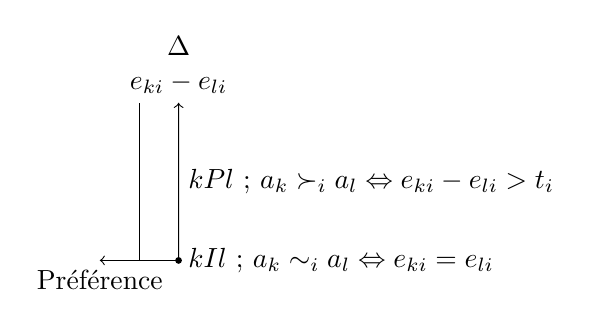
\begin{tikzpicture} %[?options?] 
%  ?tikz commands?
\draw [->] (0,0) -- (0,2);
\filldraw
(0,0) circle (1pt) --
(0,2) node[align=center, above] {$\Delta$\\$e_{ki} - e_{li}$} --
(0,1) node[align=center, right] {$kPl$ ; $a_{k} \succ_{i} a_{l} \Leftrightarrow e_{ki} - e_{li} > t_i$} --
%(0,4) circle (1pt) node[align=center, left] {t}
%(0,4) circle (1pt) node[align=center, right] {seuil entre préférence faible et préférence strict} --
%(0,3) node[align=center, right] {$kQl$ ; $ a_{k} \succsim_{i} a_{l} \Leftrightarrow q_i < e_{ki} - e_{li} \leq t_i $} --
%(0,2) circle (1pt) node[align=left, left] {q}
%(0,2) circle (1pt) node[align=left, right] {seuil entre préférence faible et indiférence}     -- 
(0,0) node[align=center, right] {$kIl$ ; $ a_{k} \sim_{i} a_{l} \Leftrightarrow e_{ki} = e_{li}$};
 %node[align=center,  above] {} --;
 \draw
 (0,0) --
 (-0.5,0)--
 (-0.5,2);
 \draw [->] (0,0) -- (-1,0);
 \filldraw 
  (-1,0) node[align=left, below] {Préférence};
 
\end{tikzpicture}
\caption{Représentation de la préférence stricte. Usage d'un critère vrai.}
\label{fig:pref_strict}
\end{figure}

Les préférences suivant un ``quasi-critère'', illustrées Fig.\ref{fig:pref_strict_distancé}, se traduisent de la façon suivante~:
\begin{equation}
\begin{cases} a_{k} \succ_{i} a_{l} \Leftrightarrow e_{ki} - e_{li} > q_i & \\
a_{k} \sim_{i} a_{l} \Leftrightarrow |e_{ki} - e_{li}| \leq q_i & 
\end{cases}
\end{equation} 
Il s'agit d'une échelle ordinale avec seuil\footnote{\blockcquote[section 3.7.1.2]{bouyssou_evaluation_2006}{Ordinal scale with a threshold}}.
La supériorité stricte de la différence des évaluations d'une alternative sur l'autre au seuil d'indifférence, lui vaut la préférence stricte. Si la différence des évaluations de deux alternatives est inférieure au seuil d'indifférence, par exemple un ordre de grandeur déterminé par un intervalle d'incertitude de l'évaluation, alors aucune des alternatives n'est préférable.

\begin{figure}
\centering
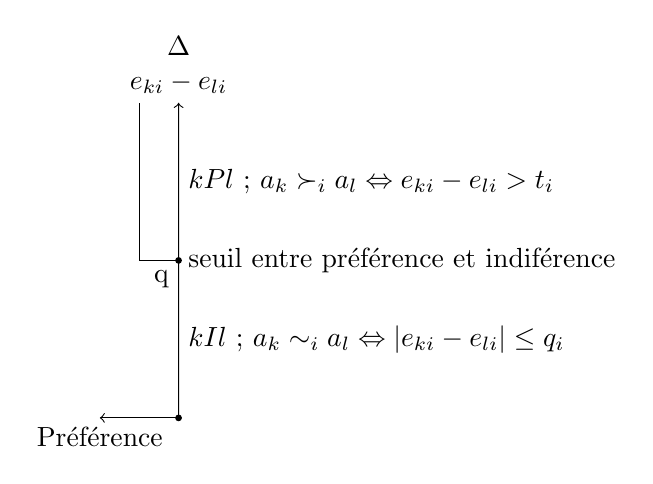
\begin{tikzpicture} %[?options?] 
%  ?tikz commands?
\draw [->] (0,0) -- (0,4);
\filldraw
(0,0) circle (1pt) --
(0,4) node[align=center, above] {$\Delta$\\$e_{ki} - e_{li}$} --
(0,3) node[align=center, right] {$kPl$ ; $a_{k} \succ_{i} a_{l} \Leftrightarrow e_{ki} - e_{li} > t_i$} --
%(0,4) circle (1pt) node[align=center, left] {t}
%(0,4) circle (1pt) node[align=center, right] {seuil entre préférence faible et préférence strict} --
%(0,3) node[align=center, right] {$kQl$ ; $ a_{k} \succsim_{i} a_{l} \Leftrightarrow q_i < e_{ki} - e_{li} \leq t_i $} --
(0,2) circle (1pt) node[align=left, below left] {q}
(0,2) circle (1pt) node[align=left, right] {seuil entre préférence et indiférence}     -- 
(0,1) node[align=center, right] {$kIl$ ; $ a_{k} \sim_{i} a_{l} \Leftrightarrow |e_{ki} - e_{li}| \leq q_i$};
 %node[align=center,  above] {} --;
  \draw
  (0,0) --
  (0,2) --
  (-0.5,2)--
  (-0.5,4);
  \draw [->] (0,0) -- (-1,0);
  \filldraw 
   (-1,0) node[align=left, below] {Préférence};
\end{tikzpicture}
\caption{Représentation de la préférence stricte avec distance. Usage de quasi-critère}
\label{fig:pref_strict_distancé}
\end{figure}

Les préférences suivant un ``pseudo-critère'', illustrées Fig.\ref{fig:weak_pref}, se traduisent de la façon suivante~\footnote{Les seuils q et t sont également exprimés en littérature par x' et x''~\cite{bouyssou_evaluation_2006}}~:
\begin{equation}
\begin{cases} a_{k} \succ_{i} a_{l} \Leftrightarrow e_{ki} - e_{li} > t_i &  \\
a_{k} \succsim_{i} a_{l} \Leftrightarrow q_i < e_{ki} - e_{li} \leq t_i & \\
a_{k} \sim_{i} a_{l} \Leftrightarrow |e_{ki} - e_{li}| \leq q_i & 
\end{cases}
\end{equation} 
%\colorbox{yellow}{probable erreur dans l'article de Rowley, relire jusqu'à validation puis mail à Hazel.}

\begin{figure}
\centering
\begin{tikzpicture} %[?options?] 
%  ?tikz commands?
\draw [->] (0,0) -- (0,6);
\filldraw
(0,0) circle (1pt) --
(0,6) node[align=center, above] {$\Delta$\\$e_{ki} - e_{li}$} --
(0,5) node[align=center, right] {$kPl$ ; $a_{k} \succ_{i} a_{l} \Leftrightarrow e_{ki} - e_{li} > t_i$} --
(0,4) circle (1pt) node[align=center, left] {t}
(0,4) circle (1pt) node[align=center, right] {seuil entre préférence faible et préférence strict} --
(0,3) node[align=center, right] {$kQl$ ; $ a_{k} \succsim_{i} a_{l} \Leftrightarrow q_i < e_{ki} - e_{li} \leq t_i $} --
(0,2) circle (1pt) node[align=left, below left] {q}
(0,2) circle (1pt) node[align=left, right] {seuil entre préférence faible et indiférence}     -- 
(0,1) node[align=center, right] {$kIl$ ; $ a_{k} \sim_{i} a_{l} \Leftrightarrow |e_{ki} - e_{li}| \leq q_i$};
 %node[align=center,  above] {} --;
 \draw
   (0,0) --
   (0,2) --
   (-0.5,2)--
   (-0.5,4)--
   (-1,4)--
   (-1,6);
   \draw [->] (0,0) -- (-1.5,0);
   \filldraw 
    (-1,0) node[align=left, below] {Préférence};
\end{tikzpicture}
\caption{Représentation de la préférence faible. Usage de pseudo-critère}
\label{fig:weak_pref}
\end{figure}
Il s'agit d'une échelle ordinale à deux seuils\footnote{\blockcquote[section 3.7.1.2]{bouyssou_evaluation_2006}{Ordinal scale with two thresholds}}.
La supériorité stricte de la différence des évaluations d'une alternative sur l'autre au seuil d'indifférence, lui vaut la préférence stricte.
La préférence faible ($\succsim$) intervient lorsque la différence des évaluations se situe entre deux seuils.
Un premier seuil peut représenter l'incertitude.
Le second peut indiquer une \emph{``distance significative''} entre les intervalles d'incertitudes.
Si la différence des évaluations de deux alternatives est inférieure au seuil d'indifférence, par exemple l'intervalle d'incertitude de l'évaluation, alors aucune des alternatives n'est jugée préférable.

Les nuances de préférences sont généralisables de façon discrète avec n seuils~\cite[3.7.1.4 Ordinal scale with k thresholds]{bouyssou_evaluation_2006}.
Les formes de préférences peuvent aussi êtres définies de façon continue (CF les dernières modalités
%de la figure~\ref{fig:pref_PROMETHEE},
dans la méthode \gls{PROMETHEE}, avec critère gaussien).

%???????????????????
%
%Autres formes de seuils, limites exclusion supérieure et inférieure
%
%? incomparabilité et ELECTRE
%
%\citetitle{roy_outranking_1991}
%\citeauthor{roy_outranking_1991}
%\cite{roy_outranking_1991}
%
%
%
%À partir des quasi- ou pseudo- critère, différentes relations de préférence peuvent être établies\blockcquote{boufateh_ben_arari_contribution_2011}{La fonction de préférence de a par rapport à b au jème critère est Fj(a,b), un nombre compris entre 0 et 1 qui croît avec l'écart gj(a) ? gj(b) en fonction de la manière dont la préférence est modélisée (figure 2.3)'']}.
%Ces relations sont également décrites par \citeauthor{deshmukh_preference_2013}.
%???????????????????

%\colorbox{red}{idem copyright à vérifier pour le cas particulier des figures, ici thèse, fr. Pas de droit US}
%\begin{figure}[h]
%\begin{center}
%%\begin{figure}[r]
%\includegraphics[width=14cm]{/home/rudy/Documents/rudy/01_These/11_production/01_COMMUNICATION/figures_extraites/Boufateh_2011_promethee_preferences.pdf}
%\caption{Formes de préférence sous PROMETHEE. Extrait de \cite{boufateh_ben_arari_contribution_2011}}
%%\end{figure}
%\label{fig:pref_PROMETHEE}
%\end{center}
%\end{figure}

%\figbox{Les lecteurs auront pu observer sur la figure\ref{fig:pref_PROMETHEE} ! \colorbox{yellow}{check rights on the graph} les parallèles de notations et descritpions de \citeauthor{bouyssou_evaluation_2006} à \citeauthor{boufateh_ben_arari_contribution_2011}.}
\subsubsection{Discussion des \textit{critères}}
Les alternatives peuvent donc être évaluées suivant des critères économiques, sociaux, de gouvernance et environnementaux, car la diversité des méthodes d'interprétation permet la prise en compte de critères (ou attributs) de natures variées.

Une grande prudence sera de mise pour la sélection ou la construction des critères.
Les critères pour être employés au sein d'une \gls{PAMC} sont de préférence~: %d'après \citeauthor{rowley_aggregating_2012} et \citeauthor{bouyssou_evaluation_2006}
``exhaustifs, en quantité minimale, monotones, cumulatifs et indépendants'', \citeauthor{rowley_aggregating_2012} citant (Bouyssou (1990)\footnote{Bouyssou, D., 1990. Building criteria: a prerequisite for MCDA. In: Bana e Costa, C.A. (Ed.), Readings in Multiple Criteria Decision Aid. Springer-Verlag, Berlin, pp. 58e80. Nous n'avons su accéder à cette référence.})\cite[p.27 (p.4 de l'article)]{rowley_aggregating_2012}.
\citeauthor{moullec_towards_2014} lorsqu'elle liste les critères indiqués par Bouyssou 1990 (semble-t-il la même référence) ne retiens que "Exhaustiveness ; Monotonicity ; Non-redundancy"~\cite{moullec_towards_2014}.

%\colorbox{yellow}{? ref bouyssou non accessible > faire un lien sur la partie de discussion des indicateurs (tous "liés et non indépendants)}
%
%
%??? Section spécifique sur les indicateurs ???
\label{sec:indépendance des indicateurs}
Plus particulièrement l'indépendance semble difficilement atteignable avec l'intégration du Life Cycle Costing et de l'\gls{ACVS}.
Rien qu'au sein du seul domaine \emph{environnemental} de l'\gls{ACV}, l'indépendance est délicate.
Peut-on sans autre précaution affirmer que l'indicateur d'épuisement des ressources d'énergie fossiles, l'indicateur de potentiel de réchauffement global et l'indicateur d'émission de particule avec son impact sur la santé humaine sont indépendants~\barre{?}~!
Sur les dimensions sociale et économique, la liaison des indicateurs est indéniable.


\exbox{
Pour reprendre la théorie de la valeur sous la formule de J.M. Jancovici, ``l'argent n'achète que des hommes''\footnote{Formule qu'il emploi dans "C'est maintenant !", co-écrit avec Alain Grandjean, 2009.}.
Considérons le cadre du travail salarié et des préférences sur les indicateurs monétaires et imaginons des alternatives parmi lesquelles il faudrait choisir.
Optons d'une part pour une \textbf{préférence décroissante de leurs coûts} respectifs (on veut acheter la moins chère).
Et d'autre part posons une \textbf{préférence croissante sur l'emploi} que les alternatives génèrent (on veut plus de travail salarié).
Cela fait apparaître par la dépendance des indicateurs une \textbf{contradiction évidente}.
Les orientations contradictoires de la préférence d'un indicateur sur l'autre sont dignes d'intérêt pour la société.
Ces deux critères sont très clairement liés par le taux horaire de rémunération applicable aux masses salariales concernées.
C'est donc le jugement de valeurs des parties prenantes qui doit faire pencher la décision vers une aire de protection (une forme de richesse ou de valeur en son sens le plus large), ou une autre.
La contradiction doit éclairer que ce qui est souhaité n'est pas la subordination (l'emploi), mais l'accès aux conditions d’existence.
Ajouter à cette première réflexion des modèles alternatifs d'obtention des condition matérielles d'existence qu'un \emph{revenu} et l'indicateur de chômage, de \emph{non-emploi}, d'\emph{absence de subordination contractualisée}, n'est plus observé avec une préférence croissante suivant la même orientation (préférence vers le moindre état de subordination).
}

Pour revenir aux caractéristiques des critères, selon \citeauthor{rowley_aggregating_2012} rappelant (\textsc{Bouyssou} 1990), il semble difficile d'obtenir \textbf{l'indépendance des critères}.
Les auteurs nous alertent sur les effets de double comptage.
Mais l'indépendance de l'ensemble des critères est-elle tout simplement nécessaire à la décision~?
Faut-il retenir la synthèse de \textsc{Moullec} ou de \textsc{Rowley} et quel éclairage pouvons nous y apporter~?
Le traitement ultérieur des critères doit être considérée pour prendre position.

\keybox{
Le fait que deux critères (corrélés ou liés causalement) évoluent de paires et dégradent un scénario considéré n'ôte pas le fait que pour ledit scénario, deux signaux négatifs \emph{sont et doivent} être perçus par les parties prenantes et le décideur.
Mais cela va plus loin.
En questionnant l'indépendance, nous nous apercevons que la redondance est question du système de valeur et non une caractéristique intrinsèque du set de critères choisi.
\textbf{Avant même leur pondération, la détermination des critères} (exhaustifs, monotones, non-redondants) \textbf{dépend donc du système de valeurs.}
}
\exbox{
Prenons deux séries d'exemples.

Si un baril de pétrole est brûlé, il réduit les ressources des générations à venir \textbf{et} engendre un forçage radiatif supplémentaire.
En suivant ces deux indicateurs (GWP, RD), fonctionnellement liés (non-indépendant), s'expriment deux conséquences négatives, significatives pour le décideur.
Bien que liées, la prise en compte de ces deux indications n'est pas un double comptage.
Les deux conséquences sont distinctes.

Considérons maintenant un indicateur tel l'énergie totale cumulée, \gls{CED}. %(CED Cumulated Energy Demand).
Employée avec un \gls{GWP} et/ou \gls{RD}, l'indication pourrait être qualifiée de redondante.
Une quantité d'énergie employée (niveau d'information "Inventaire"), n'indique en rien une conséquence (impact ou dommage).
Les trois indicateurs iront probablement de pairs.

Maintenant, si pour un système de valeur particulier, l'usage même de l'énergie est perçu comme affectant une valeur (i.e. qui génère un impact ou un dommage), alors la \gls{CED} pourrait être considérée comme non-redondante.
L'indicateur \gls{RD} se voit d'ailleurs parfois décomposé (\gls{RD} fossiles, renouvelable).
Il peut donc bien y avoir distinction de ces indicateurs corrélés sans double comptage, sous réserve de considérer les nuances attenantes.

Considérons maintenant pour seconde série, dans une même étude pour une même décision deux indicateurs~:
\begin{itemize}
\item L'impact sanitaire d'une activité (thème ``health \& safety'') au travers un indicateur social tel que proposé dans les travaux de \citeauthor{benoit-norris_identifying_2012}~\cite{benoit-norris_identifying_2012}
\item et les indicateurs de l'aire de protection ``santé humaine'' de l'\gls{ACV} tel que dans\citetitle{jolliet_impact_2003} ~\cite{jolliet_impact_2003} (par exemple)
\end{itemize}
La prise en compte simultanée des deux indicateurs engendre-t-elle un double comptage ?
Il s'agit de compartiments différents, l'ambiance de l'environnement de travail (``working environment'', indicateur sociaux ou sanitaire sur les conditions de travail) \emph{dans la techno-sphère} et l'atmosphère extérieure, représentée dans l'\gls{ACV} évaluant les échanges \emph{avec la biosphère}.
De plus il s'agit dans les deux cas de transmettre des pathologies à l'Homme.
Il y a cependant peut-être communication de l'ambiance de travail à l'environnement extérieur (aspiration pour rejet à l'atmosphère).
Ici c'est le rejet de la présence de composants de la biosphère au sein de la techno-sphère qui est problématique.
Considérer qu'il s'agit des mêmes phénomènes et que la distinction biosphère VS techno-sphère est une construction dépassée par les modèles par compartiments résout l'affaire en n'en faisant qu'un seul indicateur dont les facteurs d'impacts seront associés aux parcours et au devenir probables des substances (fate and pathways).

Toutefois si nous considérons comme situations particulières avec des facteurs tels~: \emph{l'exposition sous subordination} ; en connaissance de cause ou non ; l'exposition d'un tiers sans lien à l'activité, voir à son insu, etc. \emph{il s'agit d'indications spécifiques.}
La mesure précise par compartiment des émissions deviendra plus critique (pour éviter le double comptage ou l'absence de comptabilisation).
Bien que non-indépendants ces critères de santé considérés séparément ne sont plus \emph{redondants} entre eux.
}
%\colorbox{yellow}{? dans chap sur description et indicateurs ?}

Nous venons de le voir en exemple, le questionnement sur l'unicité, la redondance et l'indépendance nécessite une réflexion particulière.
Cette réflexion est probablement incompatible avec un processus séquentiel sans retour sur la liste de critères établis.
Ainsi, l'ordonnancement apparent des tâches avec\begin{enumerate}
\item (i) la détermination des dimensions observées et
\item (ii) la formulation des formes de préférences sur celles-ci
\end{enumerate}

reste logique mais nécessite une démarche itérative pour que les capacités cognitives humaines limitées ne réduisent pas par heuristique le nombre de dimensions observées.
Ceci nous induira lors de la reconception critique de l'ACV à réclamer~: \emph{non-pas un état fixe du système d'interprétation avant l'étude, mais sa transparence tout au long du processus.}

\subsubsection{Des méthodes d'\gls{ADMC}}
Les quasi- et pseudo- critères ainsi que les quatres relations types sont implémentés au travers des différentes versions d'outils d'\gls{ADMC}.

Citons \textsc{Promethee}
 %Preference Ranking Organization METhod For Enrichment Evaluation
 \footnote{Brans JP, Mareschal B, Vincke P. PROMETHEE: A new family of outranking methods in multicriteria analysis. JP Brans (ed), Operational Research?84, Elsevier Science Publishers BV (North-Holland); 84:408?421; 1984.}.
%\colorbox{yellow}{reprendre des références en livre bouyssou et Triantaphyllou}
Présentée par \citeauthor{deshmukh_preference_2013} dans \citetitle{deshmukh_preference_2013}, de la version I à VI il est clairement stipulé dès le résumé que~:
\blockcquote[traduction]{deshmukh_preference_2013}{
Les informations demandées par PROMETHEE sont particulièrement claires et faciles à définir pour les décideurs et les analystes.
Il s'agit de fonctions de préférence associées à chaque critère, ainsi que des poids décrivant leur importance relative.
%The information requested by PROMETHEE is particularly clear and easy to define for both decision-makers and analysts.
%It consists in a preference function associated to each criterion as well as weights describing their relative importance.
}
%\footnote{
Si \citeauthor{deshmukh_preference_2013} les qualifie de 'facile à définir', nous recommandons cependant l'usage de technique d'assistance.
Nous traiterons cela avec l'\acrshort{AHP}.
%}
%\item 

Mentionnons également \textsc{Electre}, ELimination Et Choix Traduisant la REalité\footnote{R. BENAYOUN, B. ROY, B. SUSSMANN, ELECTRE
: Une méthode pour guider le choix en présence de points de vue multiples, Note de travail n° 49 de la Direction Scientifique de la SEMA, juin 1966.},
proposé par \citeauthor{roy_classement_1968} dans \citetitle{roy_classement_1968}~\cite{roy_classement_1968}\footnote{
Développée sur une génération (68-91) \citetitle{roy_outranking_1991}~\cite{roy_outranking_1991}.}.

Ces deux familles récentes de méthodes (\textsc{Electre} et \textsc{Promethee}) nous parraissent parfaitement pertinentes pour pour les critères quantitatifs et chargés d'incertitude que nous rencontrons en \gls{ACV}.
Mais l'histoire des \gls{ADMC} n'est pas neuve et le panel de méthodes est plus varié que celles dont nous avons connaissance.
\textsc{Condorcet} (1743-1794) et son paradoxe sur les systèmes de votes font l'exemple du travail de longue date sur la thématique.
Dans le cadre de nos travaux sur la soutenabilité, \citetitle{arrow_difficulty_1950} doit être reconnue.
Dans cet article \citeauthor{arrow_difficulty_1950}
\footnote{
\blockcquote{arrow_difficulty_1950}{This paper is based on research carried on at the \textbf{RAND- Corporation}}.
Il s'agit bien des mêmes que pour la société des eaux néerlandaises.
}
énonce le Théorème d'impossibilité (ou paradoxe d'Arrow)~\cite{arrow_difficulty_1950}.
\label{Annexe:Arrow}

Le rappel de l'expression original des conditions et de l'impossibilité est fait en~\ref{Arrow},
voici leur reprise.
\begin{itemize}
\item Non-dictature~: La préférence d'un groupe d'individus n'est pas imposé par une unique personne.
\item Souveraineté~: Les préférences ne peuvent être imposées ou définie comme un ordre pré-existant.
\item Monotonie~: Il n'est pas possible de 'descendre' une alternative dans le classement par l'action d'un individu lui attribuant une importance plus 'haute'.
\item Indépendance des alternatives non-pertinentes~:
\exbox{
Pour illustrer cette condition, observons la chose suivante~:
prenons les alternatives x, y, z et w et les individus I, II et III les ordonnant avec la plus haute valeur pour la préférée.

\begin{center}
$
\begin{matrix}
      & x & y & z & w\\
I     & 4 & 3 & 2 & 1\\
II    & 4 & 3 & 2 & 1\\
III   & 2 & 1 & 4 & 3\\
Somme & 10 & 7 & 8 & 5\\
\end{matrix}
$
\end{center}

L’ordonnancement est donc x, z, y, w.

Maintenant considérons l'absence de l'alternative y.

\begin{center}
$
\begin{matrix}
      & x & z & w\\
I     & 3 & 2 & 1\\
II    & 3 & 2 & 1\\
III   & 1 & 3 & 2\\
Somme & 7 & 7 & 4\\
\end{matrix}
$
\end{center}

Il y a indétermination ou indifférence entre x et z. (ou xIz)

La condition imposée par \citeauthor{arrow_difficulty_1950} est que l'ordre x, z, w soit maintenu par l’existence antérieure de l'ordonnancement x, z, y, w.

Dans nos exercices d'\gls{ACV}, il est toutefois plus fréquent d'identifier des alternatives \textit{a posteriori} et donc d’accroître le nombre d'alternative et non de le réduire.
}
\item Universalité~: pour chaque expression de préférence identique, la solution est un unique ordre complet (pas d'indétermination).
\end{itemize}

Les suites de l’énoncé (en termes de recherche) furent de questionner chacune des conditions et sa \textit{nécessité} ainsi que les conséquences de son absence.
C'est dans la volonté d'une unique voie unanimement reconnue au sein d'un groupe qui, d'après nous, nous laisse dans l'impasse.
Nous allons traiter cette question avec une autre méthode, l'\acrshort{AHP}.

\subsubsection{Architecture des valeurs, l'\acrshort{AHP}}
\label{subsubsec:AHP}
L'\acrshort{AHP}, le processus analytique de hiérarchisation
\footnote{
Processus analytique de hiérarchisation, traduit de 'Analytic Hierarchy Process'.
Saaty, T. (1972). An eigenvalue allocation model for prioritization and planning. In Working paper, Energy Management and Policy Center: University of Pennsylvania.

Saaty, T.L., “A scaling method for priorities in hierarchical structures,” Journal of Mathematical Psychology , Vol. 15, No. 3, pp. 234-281,1977.
}
bénéficie d'un large spectre d'applications et donc du retour d'expérience attenant~\cite{vaidya_analytic_2006}
\footnote{\citeauthor{vaidya_analytic_2006}référence 150 articles d'application. Domaines d'application~: Personnel, Social, Éducation, Ingénierie, Fabrication, Industrie, Politique, Gouvernement}.
Elle a également été développé dans le cadre de décision en large groupe (LGDM large groupe decision making)~\cite{liu_method_2016}.

La méthode dans sont plus simple appareil consiste en la confrontation par paire d'éléments pour la détermination de leur importance relative.
Je présente ceci graphiquement,
inspiré par le figure aux pommes de \citeauthor{saaty_fundamentals_2004}~\cite{saaty_fundamentals_2004}, je la révise pour étendre mon propos.

Sur la base d'une échelle d'entiers allant de 1 à 9 (table~\ref{tab:saaty_echelle}), l'utilisateur oppose les composants de la paire.
\begin{table}
\centering
\caption{Échelle fondamentale\cite{saaty_decision_2004}.}
\begin{tabular}{ l l }
\hline
Valeur & Importance relative \\
\hline
1 & Égal importance  \\ 
2 & Faible \\ 
3 & Modérée \\ 
4 & Modérée plus \\ 
5 & Forte importance  \\ 
6 & Forte plus \\ 
7 & Vraiment forte ou démontrée  \\ 
8 & Vraiment plus forte \\ 
9 & Extrême importance \\ 
\hline
\end{tabular}
\label{tab:saaty_echelle}
\end{table}

\begin{figure}[htbp]
\centering
	\caption{Principe de la matrice de comparaison par paire, inspirée par \citeauthor{saaty_decision_2004}~\cite{saaty_decision_2004}}
%	\vspace{-0.2cm}
	\includegraphics[width=\linewidth]{/home/rudy/Documents/rudy/01_These/11_production/01_COMMUNICATION/figures/AHP_comparison_matrix_principle.pdf}
	\label{fig:matrix_saaty_revised}
\end{figure}
\figbox{
Les rapports d'importance dans la figure~\ref{fig:matrix_saaty_revised} se construisent de la façon suivante.

Si le réceptacle A est jugé modérément supérieur au B, le rapport C1/C2 prendra la valeur 3/1.
De façon consistante et réciproque, le rapport de C2/C1 vaudra 1/3.
etc.
}
Les priorités sont déterminées selon diverses techniques.
\citeauthor{saaty_fundamentals_2004} emploie et défend le vecteur propre principal droit (`principal right eigenvector').
Quatre méthodes sont exposées par \citeauthor{ishizaka_how_2006}\footnote{\citeauthor{barzilai_consistency_1998} propose également l'extraction de la part consistante sans révision de l'inconsistance~\cite{barzilai_consistency_1998}.} avec pour conclusion que les écarts n’apparaissent qu'entre alternatives proches et de façon croissante avec l'introduction d'inconsistance~\cite{ishizaka_how_2006}.
Ceci nous pousse à \emph{ne pas choisir une} méthode mais à les balayer ainsi qu'à explorer l'inconsistance et son origine.

La réalité ne nous permet que rarement d'être consistent.
%Reality scarcely enables us to be consistent.
		%		\includegraphics[width=0.5\linewidth]{/home/rudy/Documents/rudy/01_These/11_production/01_COMMUNICATION/figures_extraites/wikicommons/AHP/Veuve_clicquot_bottle_sizes.jpg}
%		 to 30~L for a Melchizedek or Midas of Champagne. An original standard jerrycan holds 20~L.
La problématique ne se limite pas à la critique de l'échelle numérique du classement de 1 à 9 (contenant donc beaucoup de nombres premiers pour 9 niveaux)\footnote{Il s'est avéré délicat de produire des matrices 3*3 consistantes sans (ab)user des multiples 3-6-9.}.
Ainsi, des  \href{https://en.wikipedia.org/wiki/Wine_bottle#Sizes}{bouteilles de tailles variées}, de 0.1875~L avec un piccolo à un Melchizedek ou Midas de Champagne de 30~L, comme un verre \href{http://thechive.com/2011/07/20/you-should-have-a-drink-worlds-biggest-beverages-16-photos/}{\textcolor{magenta}{pouvant contenir une personne}}, bref la distribution des entités comparées paire à paire, perturbe nos hiérarchisations.

Il y a bien entendu des développement avec préférence floue, (Fuzzy AHP)~\cite{hanine_new_2016}.
Mais ce que nous retenons des travaux de \citeauthor{saaty_decision_2004}, c'est que l’inconsistance reste utile pour développer nos systèmes de valeurs~\cite[5. From Consistency to Inconsistency]{saaty_decision_2004}.
En conséquence, plus que de réduire l'inconsistance du jugement par l'extraction d'une fraction consistante ou d'une déformation de celui-ci vers la consistance, il s'agit plus d'étendre le nombre de dimensions discutées sur la base des inconsistances remontées
\footnote{
\blockcquote[traduction]{saaty_decision_2004}{
Ainsi, nous vivons avec la contradiction que nous devons être cohérents pour capturer des connaissances valides sur le monde, mais en même temps, être prêt à changer nos états d'esprits et être inconsistant si de nouvelles informations exigent que nous pensions différemment d'auparavant.
%Thus we live with the contradiction that we must be consistent to capture valid knowledge about the world but at the same time be ready to change our minds and be inconsistent if new information requires that we think differently than we thought before.
}
}.
En somme, si nous présentons et utilisons cette méthode, ce n'est pas pour produire la sélection des alternatives, mais pour conduire une réflexion axiologique.
% Axiological thinking is not simpler.
%		
%		Not limited to AHP.
%		What matters: the 'consistence' between decision-maker's values and the used technique.

\subsection{D'autres types de méthodes~?}

\citeauthor{rowley_aggregating_2012} indique également des méthodes n'impliquant pas le décideur.
\blockcquote[traduction]{rowley_aggregating_2012}{
D'autres méthodes ont aussi été proposées qui n'impliquent pas directement le décideur, mais au lieu de cela font l'extraction un schéma de pondération inhérent aux données elles-même.
Ces méthodes 'guidées par les données' comprennent une méthode basée sur l'enveloppement des données, une méthode d'évaluation croisée (Doyle, 1995), la méthode d'entropie (pomerol et Barba-Romero, 2000) et la méthode intégrale floue (Rowley et al., Sd) .}
%Other methods have also been proposed which do not directly involve the decision maker but instead extract a weighting scheme inherent to the dataset itself. These ‘data-driven’ methods include a data envelopment analysis-based alternative cross-evaluation method (Doyle, 1995), the entropy method (Pomerol and Barba-Romero, 2000) and the fuzzy integral method (Rowley et al., n.d).}

\citeauthor*{doyle_multiattribute_1995} dans \citetitle{doyle_multiattribute_1995} propose la chose suivante.
\blockcquote[traduction]{doyle_multiattribute_1995}{
La première partie de la méthode, qui est l'application direct d'enveloppement de données, peut être pensée comme un processus idéalisé d'auto-évaluation dans laquelle chacune des alternatives pondère ses attributs afin de maximiser sa propre désirabilité par rapport aux autres alternatives.
Ces poids sont considérées comme définissant les préférences d'un fragment du marché.
La deuxième étape consiste à utiliser les poids optimaux de chaque alternative pour reconstruire l'ensemble du marché et donc de déduire la préférence d'un décideur moyen qui aurait besoin de choisir parmi ces alternatives.
}
%
%The first part of the method, wich is straightforward Data Envelopment Analysis (DEA), can be fought of as an idealized process of self-evaluation in wich each alternative weights the attributes in order to maximize its own desirability relative to the other alternatives.
%These weights are taken as defining the preferences of a fragment of the market.
%The second step is to use each alternative's optimal weights to reconstruct the entire market and thus to infer the preference of an average decision maker (DM) who needs to choose from among these alternatives.}

%Pomerol, J.-C., Barba-Romero, S., 2000. Multicriterion Decision in Management:
%Principles and Practice. Kluwer Academic Publishers, London.

%xxxxxxxxxxxxxxxxxxxxxxxxxxxxxxx

Nous marquons ici notre désaccord profond avec ces auteurs sur le propos suivant.
\blockcquote[traduction]{rowley_aggregating_2012}{
Bien que cela puisse \underline{sembler} contradictoire au but des \glspl{ADMC}, qui est d'\emph{intégrer les valeurs de décideurs}, de telles méthodes peuvent être \emph{la seule option viable si les autres méthodes sont inappropriées ou peu pratique}.
% Although this may seem to contradict one aim of MCDA, which is to incorporate decision-maker values, such methods may be the only viable option if other methods are unsuitable or impractical.
}
La praticité, (l’opérationnalité) est jugée ici supérieure à la présence effective du jugement de valeur du décideur.
Or il n'est pas question de sembler contradictoire, mais de l'être totalement.
Si le décideur sélectionné n'est pas capable de formuler ses valeurs, qu'un autre qui le sache le fasse ou que la décision soit reportée dans l'attente que la formulation puisse être faite par le décideur s'il est jugé que celui-ci est légitime.
Proposer une méthode de \emph{décision} sous des allures scientifiques, de calculs savants et complexes, qui prétende s'abstenir de jugements de valeurs \textsc{n'aide pas la prise de décision par le décideur}.
\emph{C'est la précipiter et la confisquer !}
\subsection{Des combinaisons}
Certaines techniques d'ADMC sont employées simultanément de façon à traiter une partie du processus de décision.
Ainsi, les méthodes de surclassement nécessitent comme indiqué précédemment des formes de préférences et des poids pour chaque attribut.
Une autre méthodes d'analyse multi-critère peut être employée pour déterminer la pondération des critères~\cite{myllyviita_impact_2014, kaya_integrated_2011, geldermann_fuzzy_2000}.
Pour reprendre une des conclusions de \citeauthor{herva_review_2013}, nous pouvons exploiter l'\gls{AHP} pour établir la pondération utiliser lors de la procédure de surclassement\footnote{
\blockcquote[traduction]{herva_review_2013}{
L'AHP et l'ANP étaient également très populaires, en particulier lors de la structuration d'un problème et ont souvent été utilisés comme une étape préliminaire à l'application des méthodes de surclassement et pour la détermination des poids.
%AHP and ANP were also very popular, especially when structuring a problem, and were frequently employed as a preliminary step to the application of outranking methods and for the determination of weights.
}
}.
Les travaux de \citeauthor{ziout_holistic_2014} font l'exemple de l'application de l'AHP pour la détermination de l'importance relative de critères.
\blockcquote[traduction]{ziout_holistic_2014}{
L'AHP, comme la plupart des méthodes, utilise la pondération des critères pour refléter les préférences de décision des décideurs.
L'utilisation et la sélection des poids des critères est crucial pour une bonne utilisation de la méthode (Kiritsis et al., 2003), la méthode AHP assure la bonne utilisation des poids des critères grâce à son indice de consistance (consistency index).
%AHP, as most methods, uses criteria weights to reflect decision makers preferences.
%The use and selection of criteria weights is crucial for proper use of the method (Kiritsis et al., 2003), AHP method insures the proper use of criteria weights through its consistency index.
}
Il s'agit donc ici d'une pondération par panel. % (les preneurs de décision : decision maker).
Le groupe est assisté dans sa pondération par la méthode AHP.
Dans cet article l'objectif est de choisir une option de revalorisation en fin de vie de produits (EOL end of life).
Le modèle \textsc{pestel} est exploité pour sélectionner la voie de revalorisation suivant les critères~: \textbf{P}olitiques, \textbf{É}conomiques, \textbf{S}ociaux, \textbf{T}echnologiques, \textbf{E}nvironnementaux et \textbf{L}égaux.
Toujours dans cet article la même méthode est employée pour définir le classement des scénarios de revalorisation~\cite{ziout_holistic_2014}.
\blockcquote{ziout_holistic_2014}{
L'AHP est utilisée pour classer ces options selon les multiples critères qui sont développés en section 3.3.
%AHP is used to rank these options according to multi-criteria which are developed in Section 3.3.
}
Deux méthodes d'agrégation complète successive sont donc employées.

Si comme d'autres nous employons l'\gls{AHP}, nous gardons à l'esprit les critiques qui lui sont faîtes.
\blockcquote{bouyssou_evaluation_2006}{
La technique utilisée dans AHP (Saaty, 1980), pour définir la valeur des poids est très sophistiquée (voir section 4.5.1).
Elle évite également demander au client pour les valeurs numériques, mais elle échoue pour la même raison que les méthodes précédentes.
Elle demande au client de comparer l'importance des critères. Mais le concept d'importance, même dans sa forme relative (plus important que), est si mal défini que les réponses données par le client et utilisés avec une procédure d'agrégation particulier peuvent ne pas refléter de façon fiable son système de valeurs.
Voir Belton and Gear (1983) et Dyer (1990).
%The technique used in AHP (Saaty, 1980), to set the value of the weights is very sophisticated (see section 4.5.1).
%It also avoids asking the client for numerical values, but it fails for the same reason as the previous methods.
%It asks the client to compare the importance of the criteria. But the concept of importance, even in its relative form (more important than), is so ill-defined that the answers given by the client and used with a particular aggregation procedure cannot reliably reflect his value system.
%See Belton and Gear (1983) and Dyer (1990).
}
Il semble donc nécessaire d'établir une plus ample co-élaboration des méthodes avec les psychologues.

\subsection{Interrogation perspective de travail}

%??OÙOÙOÙOÙOÙOÙOÙOÙOÙOÙOÙOÙOÙOÙOÙOÙOÙOÙOÙOÙ??

La lecture d'ouvrage de référence tel que \citetitle{bouyssou_evaluation_2006} notamment sur la préférence et sa traduction mathématique~ \cite[Chapitre 3]{bouyssou_evaluation_2006} doit nous interroger sur la possibilité (ou non) d'une réelle distinction entre observation et jugement, entre mesure et évaluation au sens de l'isolation de l'application du jugement de valeur.
Un outil intermédiaire avant même la question du jugement sera peut-être l'interrogation de la significativité des assertions.
\blockcquote[3.4. evaluation and meanigfulness]{bouyssou_evaluation_2006}{
En théorie classique de la mesure, une assertion est déclarée être significative si sa valeur vraie est inchangée lorsque les transformations admissibles sont appliquées aux échelles employées dans l'assertion.
%In classical measurement theory, an assertion is declared to be meaningful if its truth value is unchanged when admissible transformations are applied to the scales used in the assertion. 
}
Une évolution possible des travaux serait de caractériser systématiquement le type de transformation opérée et leur significativité.


%????????????????????????????????????????????????

Lors de l'étude des méthodes nous avons pu observer deux courants portant des similitudes sur des approches de détermination des valeurs.
En effet, la description de certaines méthodes mentionne que hors des alternatives, il est difficile de définir les préférences sur les indicateurs.
C'est la question des 'préférences exprimées' et 'préférences révélées', en trame de fond de la monétarisation.
La réflexion axiologique pour l'élicitation et l'articulation des valeurs nécessitera certainement de nombreuses boucles en un processus long et continu.


%\colorbox{yellow}{à relocaliser !}
La non-compensation nécessaire au concept de soutenabilité forte semble exclure des méthodes disponibles celles d'agrégation complète pour la sélection du choix final.
Toutefois, ne peut-on pas élargir nos possibilités ?
Posons des scores uniques (résultat agrégés) de différentes alternatives égaux (mathématiquement) comme incomparable (sémantiquement).
Y'aurait-il une décision finale différente, sur la base d'une même caractérisation et de poids identiques, interprétée suivant des agrégations partielles et complètes ?
\begin{figure}[htbp]
\centering
	\caption{Préférences et perspectives}
%	\vspace{-0.2cm}
	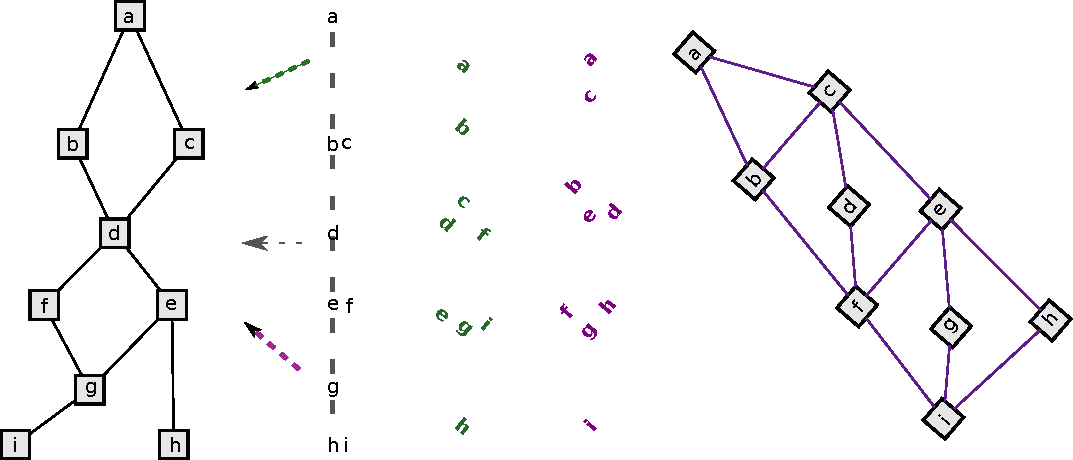
\includegraphics[width=0.7\linewidth]{/home/rudy/Documents/rudy/01_These/11_production/01_COMMUNICATION/figures/preferences_reseau_perspectives.pdf}
	\label{fig:preferences_perspectives}
\end{figure}
\figbox{
Lecture, de la représentation Fig.\ref{fig:preferences_perspectives}.
Dans quelle mesure des techniques différentes (agrégation complète, liste ordonnée ou réseau de préférences) et des perspectives différentes (figurativement avec l'inclinaison du réseau) ) modifient-elles les relations perçues entre entités et les décisions consécutives ?
Dans quelle mesure la perspective choisie sur les relations entre entités affecte-t-elle la décision\footnote{Il s'agit évidement d'une représentation figurative, les n dimensions alimentant la préférence ne sont pas réductibles à un plan de deux dimensions.} ?
Quelle est la réduction d'information minimale possible sans dépasser les seuils cognitifs et psychologiques ni déformé de façon inconsistante le jugement du décideur?
}


%\colorbox{yellow}{vers chap 4-5}

%\colorbox{yellow}{Reprendre exemple minimal avec le MMC1 de Rowley énergie coût}

%Il faut différencier les agrégations complètes pour le déterminer.
%\begin{itemize}
%\item Somme pondérée des indicateurs normalisés
%\begin{itemize}
%\item avec normalisation interne
%\item avec normalisation externe
%\end{itemize}
%\end{itemize}
%
%Cette analyse permettrait d'intégrer dans le corpus d'études soutenant la thèse d'une soutenabilité forte, des travaux sur des ''index`` de soutenabilité.
%Où comment concentrer l'information sur un indicateur unique ?
%Cela bien-sur est fait avec un grand nombre de dimensions.
%
%=> somme pondérée face à promethee face à AHP
%pressage de thèses :
%
%Moullec ? Génération de solution

Nous avons vu que l'intégration du jugement du décideur est un élément clef.
Pour présenter la question de la pluralité du corps décisionnaire, nous nous penchons sur les travaux d'\citeauthor{adla_aide_2010}.
Sans développer l'ensemble du contenu de \citetitle{adla_aide_2010}, nous observerons que la réussite d'un groupe vaste réside dans la maîtrise des communications synchrone, asynchrone, localisée et distribuée\footnote{Figure 3.3 : Quatre combinaisons des systèmes d’aide à la décision de groupe [Grudin 94], dans le Temps et l'espace~\cite{adla_aide_2010}}.

La prise en compte des parties prenantes visant la soutenabilité à l'échelle globale, tout en leur garantissant la protection de l'anonymat, \emph{est} la problématique du vote à distance (électronique).
Transparence, confidentialité, anonymat, unicité, sincérité, nous pourrions mettre tous ceci dans le cadre de l'expression du système de valeur pour la décision.
Et nous n'aurions aucun mal à reconnaître des travaux comme \citetitle{enguehard_vote_2007} de \citeauthor{enguehard_vote_2007}~\cite{enguehard_vote_2007} dans notre champ disciplinaire (ou interdisciplinaire).

La problématique de l'expression non biaisée dans les groupes distribués reste selon nous la question de `l'anonymisation-vérifiabilité' qui n'a pu être résolue jusqu'ici~\cite{pellegrini_chaines_2014}.
Il semble donc que notre espèce ne puisse accéder à ce stade de rationalité qu'en modifiant son comportement face aux expressions et au respect des opinions de chacun.e.s, pour accéder à la déclaration nominative.
Il serait naïf d'écrire cela ici sans ajouter qu'une telle occurrence est peu probable sans une horizontalisation des pouvoirs permettant de ne plus craindre d'action contre ces expressions d'opinions.
Par exemple, l'universalisation du salaire, libère de la contrainte à l'accès aux conditions matérielles d'existence.
Le tirage au sort aux fonctions de gouvernance (du local jusqu'au supra-national, tous pouvoirs confondus), libère des pressions des luttes partisanes et électives.
La co-propriété d'usage des moyens de production, libère de la subordination quant aux finalités et moyens choisis pour les obtenir.
Ne resterait donc que la coercition physique directe, difficilement extensible à de large ensemble (sous réserve des mécanismes cités précédemment).
Ces artefacts ne sont pas encore universellement appliqué ni reconnu.
Nous n'y sommes donc pas encore.


\subsection{Conclusion sur l'ADMC}
\label{concl:mcdm}

Nous avons vu au travers de cette présentation la diversité des méthodes disponibles, leurs caractéristiques et les fondements de l'\gls{ADMC}.
Nous avons ensuite traité la question des indicateurs (construction des critères) ainsi que leur formes d'agrégation, complète et partielle.
Nous en sommes venu au fait que la confrontation des deux approches doit distinguer les concepts faible et fort de la soutenabilité.
Mais en définitive, l'action de décision réside dans la mise en œuvre d'une unique alternative.
Même s'il peut s'agir de la combinaison d'alternatives, la combinaison elle-même reste une alternative unique.

La confrontation de l'école américaine et de l'école européenne (AHP, ELECTRE) est décrite par \citeauthor{lootsma_french_1990}~\cite{lootsma_french_1990}.
Elle relève par négatif les incohérences relatives aux approches de "l'évaluation objective".
C'est une indication sur l'acceptabilité de la subjectivité que nous retiendrons donc ici en conclusion.
\blockcquote[traduction]{lootsma_french_1990}{
La RAND Corporation, par exemple, une grande société de conseil américaine commanda le projet PAWN (pion) (analyse des politiques de gestion de l'eau pour les Pays-Bas, CF rapports de PAWN, 1981-1983) par l'autorité de gestion de l'eau néerlandaise `Rijkswaterstaat'
[.Elle (RAND)] a conçu un grand nombre de stratégies alternatives pour le contrôle des eaux de surface.
\emph{Ils ont rejeté l'analyse multi-critère pour la sélection finale d'une stratégie particulière, au motif que les décideurs devraient s'accorder explicitement sur les poids des critères et sur les scores des impacts.}
%The RAND Corporation, for instance, a large American consulting company commissioned with the PAWN project (Policy Analysis of Water Management for the Netherlands, see the PAWN reports, 1981-1983) by the Dutch water management authority Rijkswaterstaat, designed a large number of alternative stratégies for surface-water control.
%\emph{They rejected multi-criteria analysis for the final sélection of a particular strategy, on the ground that the decision makers would have to agree explicitly on the criterion weights and on the impact scores.
}
\keybox{
Ce qui fait obstacle à plus de rationalité dans les décisions humaines serait donc semble-t-il qu'il faille pour le décideur, être en accord avec son propre système de valeur et (pouvoir) l'assumer pleinement.
}
Toutefois, se maintenir dans l'irrationalité volontairement peut être d'autant plus préjudiciable que la solution sélectionnée peut être plus 'loin' (avec le système de valeur implicite), d'une solution plus rationnellement choisie avec le système de valeur explicite controversé mais transparent, comme d'un système plus consensuel ou d'un compromis explicité.

\keybox{
C'est en somme, au delà de l'acceptabilité de la complexité, une question de la légitimité du système de valeurs du décideur qu'il convient de résoudre pour que les \gls{ADMC}, de façon générale, et donc l'\gls{ACV} de façon particulière, soient acceptées.
}